\icode{E-MD-CA-L3-261120-003}
如图所示，质量 \(m =\) \,\qty{10}{kg}的小球挂在倾角 \(\theta =\) \,\qty{37}{\degree}，质量 \(M =\) \,\qty{40}{kg}的光滑倾斜面的固定铁杆上，求：
\begin{enumerate}
	\item 为了使小球不飞起来，斜面水平加速度最大是多少？
	\item 当斜面和小球都以 \(a_1 = 0.5g\) 的加速度向右匀加速运动时，小球对绳的拉力和对斜面的压力分别为多少？
	\item 当斜面和小球都以 \(a_2 = \sqrt{3}g\) 的加速度向右匀加速运动时，小球对绳的拉力和对斜面的压力又是分别是多少？
\end{enumerate}

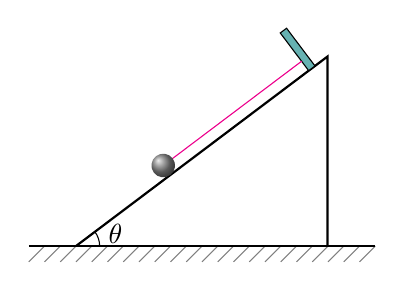
\begin{tikzpicture}
	\begin{scope}[rotate=37]
		\draw[thick] (0,0)--(4,0)--++(-127:2.4);
		\draw[fill=teal!60] (3.7,0) rectangle(3.8,.6);
		\draw[magenta] (3.7,.15)--(1.5,.15);
		\shade[ball color=gray] (1.5,.15) circle(.15);
	\end{scope}
	\draw (.3,0) arc(0:37:.3);
	\node at(.5,.16){\(\theta\)};
	\foreach \x in {-.6,-.4,...,3.8}
		\draw[gray] (\x,-.2)--++(.2,.2);
	\draw[thick] (-.6,0)--(3.8,0);
\end{tikzpicture}
\begin{answer}
	
\end{answer}